%----------------------------------------------------------------------------------------
%	PACKAGES AND OTHER DOCUMENT CONFIGURATIONS
%----------------------------------------------------------------------------------------

\documentclass[twoside,twocolumn,a4paper]{article}

\usepackage{blindtext} % Package to generate dummy text throughout this template 

\usepackage[T1]{fontenc} % Use 8-bit encoding that has 256 glyphs

\usepackage{lmodern}

\usepackage[hyphenbreaks]{breakurl}

\usepackage[hyphens]{url}

%\usepackage[super,sort&compress]{natbib}
%\usepackage{natbib}
%\setlength{\bibsep}{0.0pt}

\usepackage{graphicx}

\linespread{1.05} % Line spacing - Palatino needs more space between lines
\usepackage{microtype} % Slightly tweak font spacing for aesthetics

\usepackage[spanish]{babel} % Language hyphenation and typographical rules

\usepackage[numbib,notlof,notlot,nottoc]{tocbibind} % Shows bibliography as a section

\usepackage[hmarginratio=1:1,top=32mm,columnsep=20pt]{geometry} % Document margins

\usepackage[hang, small,labelfont=bf,up,textfont=up]{caption} % Custom captions under/above floats in tables or figures

\usepackage{booktabs} % Horizontal rules in tables

\usepackage{enumitem} % Customized lists

\setlist[itemize]{noitemsep} % Make itemize lists more compact

\usepackage{abstract} % Allows abstract customization

\renewcommand{\abstractnamefont}{\normalfont\bfseries} % Set the "Abstract" text to bold

\usepackage{fancyhdr} % Headers and footers
\pagestyle{fancy} % All pages have headers and footers
\fancyhead{} % Blank out the default header
\fancyfoot{} % Blank out the default footer
\fancyhead[C]{Laboratorio 3 $\bullet$ Informe 2 $\bullet$ Grupo 8: Inafuku, Petino, Poggi} % Custom header text
\fancyfoot[C]{\thepage} % Custom footer text

\usepackage{titling} % Customizing the title section

\usepackage{hyperref} % For hyperlinks in the PDF

%----------------------------------------------------------------------------------------
%	TITLE SECTION
%----------------------------------------------------------------------------------------

\setlength{\droptitle}{-4\baselineskip} % Move the title up

\pretitle{\begin{center}\LARGE\bfseries} % Article title formatting
\posttitle{\end{center}} % Article title closing formatting
\title{Caracterizaci\'on de diodos. Rectificadores de media y onda completa.} % Article title
\author{%
\textsc{Maximiliano Inafuku} \\[1ex] % Your name
\normalsize \href{mailto:maxi-46@hotmail.com}{maxi-46@hotmail.com} % Your email address
\and % Uncomment if 2 authors are required, duplicate these 4 lines if more
\textsc{Ernesto Petino} \\[1ex] % Second author's name
\normalsize \href{mailto:ernesto.atmo@gmail.com}{ernesto.atmo@gmail.com} % Second author's email address
\and % Uncomment if 2 authors are required, duplicate these 4 lines if more
\textsc{Ignacio Poggi} \\[1ex] % Second author's name
\normalsize \href{mailto:ignaciop.3@gmail.com}{ignaciop.3@gmail.com} % Second author's email address
}

\date{Grupo 8 - Laboratorio 3, C\'atedra Bilbao - Departamento de F\'isica, Facultad de Ciencias Exactas y Naturales, Universidad de Buenos Aires \newline \\ \today} % Leave empty to omit a date
\renewcommand{\maketitlehookd}{%
\begin{abstract}
\noindent En este trabajo se arm\'o un circuito electr\'onico simple para medir la resistencia de una l\'ampara incandescente. Se analizaron los datos obtenidos con el programa Origin 8.5 y se realizaron ajustes lineal, cuadr\'atico y c\'ubico. Se encontr\'o que el mejor ajuste para los datos obtenidos es el cuadr\'atico con sus par\'ametros libres ($R^2$ = 0,99999), dado que la resistencia de la l\'ampara se ve afectada por la intensidad de corriente que la atraviesa, as\'i como tambi\'en la temperatura de su filamento y la del ambiente.
\end{abstract}
}

%----------------------------------------------------------------------------------------

\begin{document}

% Print the title
\maketitle

%----------------------------------------------------------------------------------------
%	ARTICLE CONTENTS
%----------------------------------------------------------------------------------------

\section{Introducci\'on}

El diodo es un dispositivo de dos terminales que permite el paso de la corriente en una sola direcci\'on. Los m\'as utilizados actualmente son los diodos semiconductores y Zener (Figura \ref{fig:tipos_diodos}).\par

Cuando se somete al diodo semiconductor a una diferencia de tensi\'on externa, puede polarizarse de forma directa o inversa. En la polarizaci\'on directa, la bater\'ia disminuye la barrera de potencial, permitiendo el paso de la corriente de electrones a trav\'es de la uni\'on; es decir, el diodo polarizado directamente conduce la electricidad. En el caso de la polarizaci\'on inversa, el polo negativo de la bater\'ia se conecta a la zona p y el polo positivo a la zona n, lo que hace aumentar la zona de carga, y la tensi\'on en dicha zona hasta que se alcanza el valor de la tensi\'on de la bater\'ia. \par

Otro tipo de diodo estudiado es el diodo Zener. Estos se emplean para producir una tensi\'on entre sus terminales muy constante y relativamente independiente de la corriente que los atraviesan. Normalmente, polarizados en forma inversa no permite pr\'acticamente el pasaje de corriente, pero al alcanzar una determinada tensi\'on (tensi\'on Zener), se produce un aumento de la cantidad de corriente que lo atraviesa, manteniendo la tensi\'on entre sus terminales pr\'acticamente constante.

\begin{figure}[h]
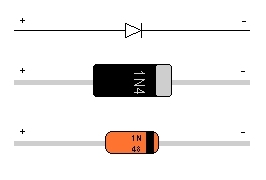
\includegraphics[width=\linewidth]{tipos_diodos.jpg}
\caption{Clases de diodos estudiados. De arriba hacia abajo: diagrama de un diodo, diodo semiconductor y diodo Zener.}
\label{fig:tipos_diodos}
\end{figure}

El modelo utilizado para caracterizar al diodo es el de Shockley, el cual permite aproximar el comportamiento del mismo en la mayor\'ia de los circuitos. La ecuaci\'on que relaciona la intensidad de corriente y la diferencia de potencial es \cite{eq:shockley}:
\begin{equation}
\label{eq:shockley}
I = I_{S}(e^\frac{V_{D}}{nV_{T}} - 1)
\end{equation}

donde

\begin{itemize}
\item 
$V_{D}$: Tension a trav\'es del diodo. 
\item 
$I_{S}$: Intensidad de corriente de saturaci\'on que se establece al polarizar inversamente el diodo ($\sim 10^{-12}$ A).
\item
$V_{T}$: Tension t\'ermica ($\sim$ 25 mV a 25�C). Se define como $\frac{kT}{q}$, donde $k$ es la constante de Boltzmann, $T$ la temperatura y $q$ la carga del electr\'on.
\item
$n$: Factor de calidad.  
\end{itemize}

La ecuaci\'on (\ref{eq:shockley}) da lugar a una curva caracter\'istica (Figura \ref{fig:curva_shockley}) con los siguientes par\'ametros:

\begin{itemize}
\item 
$V_{u}$: Tensi\'on umbral. Al polarizar directamente el diodo, la barrera de potencial inicial se va reduciendo, incrementando la corriente ligeramente. Sin embargo, cuando la tensi\'on externa supera la tensi\'on umbral, la barrera de potencial desaparece.
\item 
$I_{max}$: Intensidad de corriente m\'axima que puede conducir el diodo sin fundirse.
\item
$V_{r}$: Tensi\'on de ruptura. A partir de un determinado valor de la tensi\'on, el diodo comienza a conducir tambi\'en en polarizaci\'on inversa. 
\end{itemize}

\begin{figure}[h]
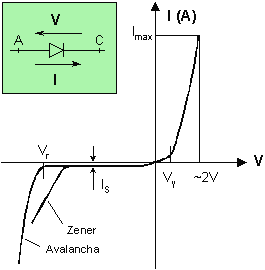
\includegraphics[width=\linewidth]{curva_shockley.jpg}
\caption{Curva caracter\'istica de un diodo seg\'un el modelo de Shockley.}
\label{fig:curva_shockley}
\end{figure}


\textbf{Rectificadores de media onda y onda completa.} \newline
\par
Los rectificadores el\'ectricos son los circuitos encargados de convertir la corriente alterna en corriente continua. Los m\'as habituales son los construidos con diodos. Los dos tipos de rectificadores estudiados en este trabajo son los rectificadores de media onda y los rectificadores de onda completa. \par

Los rectificadores de media onda funcionan haciendo pasar la mitad de la corriente alterna a trav\'es de uno o m\'as diodos, convirtiendo en este paso dicha mitad de la corriente alterna en corriente el\'ectrica directa. Estos rectificadores no son muy eficientes porque s\'olo convierten la mitad de la corriente alterna en corriente directa; por lo tanto, solo un diodo es necesario para su funcionamiento.\par

Los rectificadores de onda completa son m\'as complejos que los rectificadores de media onda, pero tambi\'en son mucho m\'as eficientes. Estos generalmente utilizan cuatro diodos para funcionar (puente de diodos), haciendo pasar la corriente alterna a trav\'es de dicho puente, obteniendo un terminal positivo y otro negativo, caracter\'istico de la corriente directa.


%------------------------------------------------

\section{Dispositivo experimental}


%------------------------------------------------
\section{Resultados y an\'alisis}

%------------------------------------------------

\section{Conclusiones}


%----------------------------------------------------------------------------------------
%	REFERENCE LIST
%----------------------------------------------------------------------------------------

\begin{thebibliography}{99} % Bibliography - this is intentionally simple in this template

\bibitem{eq:potencial} E. M. Purcell, \textit{Electricidad y Magnetismo - Berkeley Physics Course Vol. 2}, Editorial Revert\'e S.A., 2da edici\'on, Barcelona (1988), p\'ag. 124
\bibitem{eq:ohm1} E. M. Purcell, \textit{Electricidad y Magnetismo - Berkeley Physics Course Vol. 2}, Editorial Revert\'e S.A., 2da edici\'on, Barcelona (1988), p\'ag. 124
\bibitem{eq:ohm2} E. M. Purcell, \textit{Electricidad y Magnetismo - Berkeley Physics Course Vol. 2}, Editorial Revert\'e S.A., 2da edici\'on, Barcelona (1988), p\'ag. 123
\bibitem{Fuente} \url{http://goo.gl/lu3XiA}
\bibitem{amp} \url{http://goo.gl/hgNeqO}
\bibitem{volt} \url{http://goo.gl/BlIRc2}
 
\end{thebibliography}

%----------------------------------------------------------------------------------------

\end{document}